\subsection{Benchmarks}

In this subsection, we present benchmarks with the GPU that compare the performance of various computational tasks. The goal is to provide a detailed analysis of the time processes involved and to draw meaningful conclusions about the performance characteristics of the GPU.

\begin{center}
   \textbf{Benchmark Methodology}
\end{center}

The benchmarks conducted are designed to evaluate the performance of GPU computations to see the differences against the CPU performance. To ensure a fair comparison, the same set of algorithms and operations are executed on both types of hardware, so in this subsection it's going to be analyzed similar benchmarks to the CPU ones. The benchmarks focus on evaluating:

\begin{itemize}
    \item \textbf{Execution Time:} The time taken to complete the computations on each platform.
    \item \textbf{Scalability:} How performance scales with increasing problem size and complexity.
    \item \textbf{Efficiency:} The computational efficiency of the operations, including memory usage and processing power.
\end{itemize}

% \subsubsection{Benchmark Configuration}

% To accurately assess performance, the following steps were taken:

% \begin{itemize}
%     \item \textbf{Code Consistency:} The same algorithms were implemented for both CPU and GPU. This included tasks such as matrix multiplications, vector operations, and other common benchmarks.
%     \item \textbf{Optimization:} Both the CPU and GPU code were optimized according to their respective best practices. For CPU, this involved tuning compiler flags and utilizing multi-threading capabilities. For GPU, this included optimizing memory access patterns and utilizing parallel processing effectively.
%     \item \textbf{Environment:} Benchmarks were conducted in a controlled environment to minimize variability. The hardware specifications, such as CPU model and GPU model, were kept consistent across tests.
% \end{itemize}

\subsubsection{Simply GPU Matrix Multiplication}

This subsection presents a simple benchmark for evaluating the performance of matrix multiplication on the GPU. The objective is to measure the time taken for matrix multiplication using GFlops with varying matrix sizes. The benchmark uses the Julia programming language and the CUDA library.

The code below performs matrix multiplications for matrices of different sizes and records the time taken for each operation. The results are printed to the console, providing an overview of how the execution time scales with matrix size.

\begin{center}
   \textbf{Description of the Benchmark}   
\end{center}

\begin{enumerate}
   \item \textbf{Matrix Size Variation:} The benchmark tests matrix sizes ranging from 100 to 10,000 in increments of 100.
   \item \textbf{Matrix Initialization:} For each size \(N\), two matrices \(A\) and \(B\) are initialized with random floating-point values using the `CUDA.rand` function.
   \item  \textbf{Timing Measurement:} The time required for matrix multiplication \(A \times B\) is measured using the `CUDA.@elapsed` macro. This provides the duration of the multiplication operation.
   \item  \textbf{Results Output:} The matrix size \(N\) and the corresponding duration \(t\) are printed to the console. The results can be saved to a CSV file, although the line for writing to the file is commented out in this example.
\end{enumerate}

\begin{figure}[h]
    \begin{center}
        % Recommended preamble:
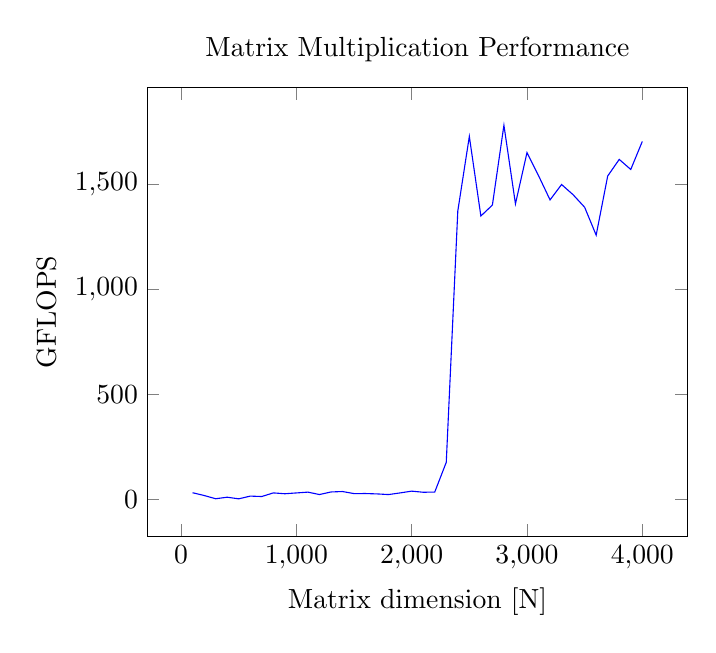
\begin{tikzpicture}
\begin{axis}[xlabel={Matrix dimension [N]}, ylabel={GFLOPS}, title={Matrix Multiplication Performance}]
    \addplot[no marks, blue]
        table[row sep={\\}]
        {
            \\
            100.0  33.10381281366246  \\
            200.0  19.879135192021558  \\
            300.0  4.476982156021999  \\
            400.0  11.709601500926066  \\
            500.0  4.020430193911908  \\
            600.0  17.013146648014878  \\
            700.0  14.998810240130217  \\
            800.0  32.22168459738295  \\
            900.0  28.238231464685082  \\
            1000.0  32.058383455759724  \\
            1100.0  35.91166448314556  \\
            1200.0  24.450673633047973  \\
            1300.0  36.695108185333  \\
            1400.0  38.835771390634285  \\
            1500.0  28.887190659163995  \\
            1600.0  29.233355263905146  \\
            1700.0  27.429380899156925  \\
            1800.0  24.321635544065924  \\
            1900.0  32.22105620285489  \\
            2000.0  40.627151940613494  \\
            2100.0  35.36037303883538  \\
            2200.0  36.194792483175625  \\
            2300.0  177.81721788465265  \\
            2400.0  1373.6961997214185  \\
            2500.0  1728.7474836007068  \\
            2600.0  1350.0127653040865  \\
            2700.0  1402.0700430511176  \\
            2800.0  1782.003309142992  \\
            2900.0  1407.8131252123346  \\
            3000.0  1651.613678544608  \\
            3100.0  1542.278774806327  \\
            3200.0  1426.756167615151  \\
            3300.0  1499.9349653079307  \\
            3400.0  1451.2283947671754  \\
            3500.0  1391.7504574757231  \\
            3600.0  1258.980438563542  \\
            3700.0  1540.3434204700604  \\
            3800.0  1619.399732580744  \\
            3900.0  1571.5020221428958  \\
            4000.0  1704.646186876883  \\
        }
        ;
\end{axis}
\end{tikzpicture}

   \end{center}
   \caption{GPU efficiency with matrix multiplications.}
   \label{}
\end{figure}

\paragraph{Code}

Here is the Julia code used for this benchmark:

\begin{comment}
\lstinputlisting[language=Julia]{code/1/matrix_mult.jl}
\end{comment}

\begin{lstlisting}[language=Julia]
using LinearAlgebra

# Function to initialize random matrices
function matrix_initialization(N)
    A = rand(Float32, N, N)
    B = rand(Float32, N, N)
    return A, B
end

# Function to perform matrix multiplication using the built-in Julia method
function matrix_multiplication(A, B)
    return A * B
end

# Custom matrix multiplication method with a manual loop
function custom_matrix_multiplication(A, B)
    (N, M) = size(A)
    (M, L) = size(B)
    C = zeros(Float32, (N, L))

    for i in 1:N, j in 1:L
        for k in 1:M
            C[i, j] += A[i, k] * B[k, j]
        end
    end
    return C
end

# Transpose optimization for more efficient memory access
function optimized_matrix_multiplication(A, B)
    (N, M) = size(A)
    (M, L) = size(B)
    BT = transpose(B)
    C = zeros(Float32, (N, L))

    for k in 1:M
        for j in 1:L, i in 1:N
            C[i, j] += A[i, k] * BT[j, k]
        end
    end
    return C
end

# Example usage
N = 500
A, B = matrix_initialization(N)

# Built-in matrix multiplication
C_builtin = matrix_multiplication(A, B)

# Custom matrix multiplication
C_custom = custom_matrix_multiplication(A, B)

# Optimized matrix multiplication
C_optimized = optimized_matrix_multiplication(A, B)

println("Matrix multiplication complete.")
\end{lstlisting}



\subsubsection{Matrix Multiplication Modifying N using Times}

In this subsection, we present a benchmark that measures the performance of matrix multiplication on the GPU. Specifically, we analyze the duration required for matrix multiplication as the size of the matrices varies. The benchmark is conducted using the Julia programming language with the CUDA library.

The benchmark procedure involves varying the size of the matrices and recording the time taken for a series of matrix multiplications. The results are then saved to a CSV file for further analysis.

\begin{center}
   \textbf{Description of the Benchmark}   
\end{center}

\begin{enumerate}
   \item \textbf{Matrix Size Variation:} The benchmark varies the size of the matrices from 300 to 2499 with a step size of 25.
   \item \textbf{Number of Operations:} For each matrix size \(N\), the number of operations `TIMES` is calculated to ensure that the total number of operations is constant for different matrix sizes. The formula used is:
   \[
   \text{TIMES} = \frac{N_{\text{ops}}}{2 \times N^3}
   \]
 where \(N_{\text{ops}}\) is set to \(2 \times 10000^3\).
   \item \textbf{Timing Measurement:} The time taken to perform the matrix multiplications is measured using the `@elapsed` macro. The benchmark performs `TIMES` multiplications and records the total duration.
   \item \textbf{Data Recording:} The results, including matrix size, number of operations, and duration, are written to a CSV file for analysis.
\end{enumerate}

\begin{figure}[h]
   \begin{center}
       % Recommended preamble:
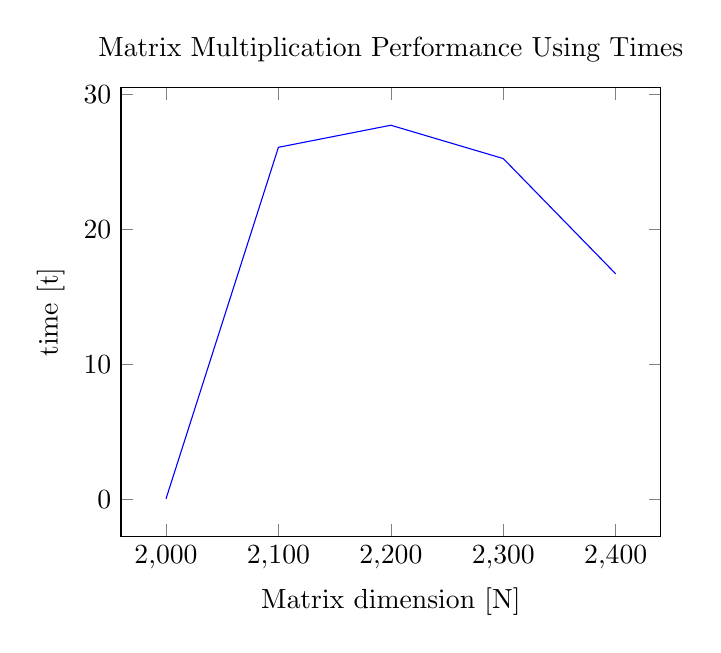
\begin{tikzpicture}
\begin{axis}[xlabel={Matrix dimension [N]}, ylabel={time [t]}, title={Matrix Multiplication Performance Using Times}]
    \addplot[no marks, blue]
        table[row sep={\\}]
        {
            \\
            2000.0  0.0251821  \\
            2100.0  26.065924  \\
            2200.0  27.701773  \\
            2300.0  25.231264  \\
            2400.0  16.692413  \\
        }
        ;
\end{axis}
\end{tikzpicture}

  \end{center}
  \caption{GPU efficiency with matrix multiplications.}
  \label{}
\end{figure}
\newpage

\paragraph{Code}

Below is the Julia code used to perform this benchmark:

\begin{comment}
\lstinputlisting[language=Julia]{code/2/matrix_mult_times.jl}
\end{comment}

\begin{lstlisting}[language=Julia]
using LinearAlgebra, CPUTime

# Function to initialize random matrices
function matrix_initialization(N)
    A = rand(Float32, N, N)
    B = rand(Float32, N, N)
    return A, B
end

# Function to perform matrix multiplication using the built-in Julia method
function matrix_multiplication(A, B)
    return A * B
end

# Custom matrix multiplication method with a manual loop
function custom_matrix_multiplication(A, B)
    (N, M) = size(A)
    (M, L) = size(B)
    C = zeros(Float32, (N, L))

    for i in 1:N, j in 1:L
        for k in 1:M
            C[i, j] += A[i, k] * B[k, j]
        end
    end
    return C
end

# Function to measure execution time of matrix multiplication
function measure_execution_time(N, matmul_func)
    A, B = matrix_initialization(N)
    start_time = time_ns()
    matmul_func(A, B)
    elapsed_time = (time_ns() - start_time) / 1e9  # Convert from nanoseconds to seconds
    return elapsed_time
end

# Example usage
N = 500
time_builtin = measure_execution_time(N, matrix_multiplication)
time_custom = measure_execution_time(N, custom_matrix_multiplication)

println("Execution time for built-in matrix multiplication: ", time_builtin, " seconds")
println("Execution time for custom matrix multiplication: ", time_custom, " seconds")
\end{lstlisting}


\newpage

\subsubsection{GPU Matrix Multiplication Performance GFLOPS}

This subsection describes a benchmark that measures the performance of matrix multiplication on the GPU using an NVIDIA GeForce GTX 1060 6GB. The objective is to evaluate the time taken for matrix multiplication across various matrix sizes and compare it to theoretical performance estimates. The benchmark uses the Julia programming language along with the CUDA and Plots libraries.

The following Julia code performs the matrix multiplication and measures the execution time. It also plots the performance results in GFLOPS (Giga Floating Point Operations per Second) to visualize how the GPU handles different matrix sizes.

\begin{center}
   \textbf{Description of the Benchmark}   
\end{center}

\begin{enumerate}
   \item \textbf{Matrix Initialization:} The matrix initialization GPU function initializes matrices \(A\) and \(B\) with random floating-point values and transfers them to the GPU as `CuArray`.
   \item \textbf{Matrix Multiplication:} The matrix multiplication function performs matrix multiplication on the CPU, while the matrix multiplication GPU function measures the time required for GPU-based matrix multiplication using the `CUDA.@elapsed` macro.
   \item \textbf{Timing Measurement:} The time matrix multilication function measures the duration of matrix multiplications for different matrix sizes \(N\). It calculates the time per operation and compares it to theoretical performance estimates.
   \item \textbf{Results Plotting:} The plot results function generates a plot of the GPU performance in GFLOPS versus matrix size \(N\). It also includes a label indicating the maximum GFLOPS achieved.
   \item \textbf{Data Analysis:} The benchmark results are printed to the console and visualized using the `Plots` library. The maximum GFLOPS achieved is highlighted in the plot for comparison with theoretical performance.
\end{enumerate}

\begin{figure}[h]
   \begin{center}
      % Recommended preamble:
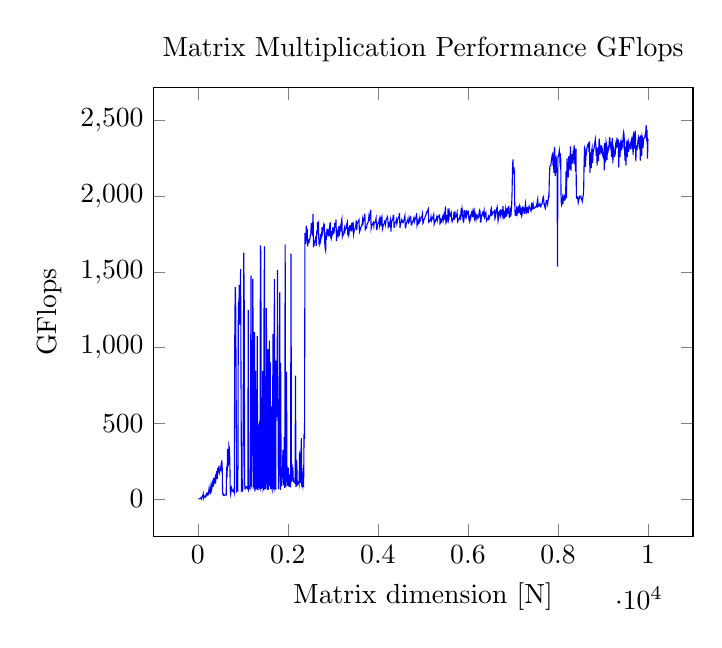
\begin{tikzpicture}
\begin{axis}[xlabel={Matrix dimension [N]}, ylabel={GFlops}, title={Matrix Multiplication Performance GFlops}]
    \addplot[no marks, blue]
        table[row sep={\\}]
        {
            \\
            10.0  0.00011007457552491813  \\
            20.0  0.0041866185205536805  \\
            30.0  0.33707865168539325  \\
            40.0  0.9391049156272927  \\
            50.0  2.9308323563892147  \\
            60.0  4.337349397590361  \\
            70.0  7.563395810363837  \\
            80.0  0.4191053083943846  \\
            90.0  13.651685393258427  \\
            100.0  18.709073900841908  \\
            110.0  14.107048224695282  \\
            120.0  31.446769790718836  \\
            130.0  4.416968234821069  \\
            140.0  13.921867072552002  \\
            150.0  16.70378619153675  \\
            160.0  19.87867022567338  \\
            170.0  11.52745190051619  \\
            180.0  13.864257696422204  \\
            190.0  34.45867872393871  \\
            200.0  31.527093596059117  \\
            210.0  36.41045803027325  \\
            220.0  23.968486212718062  \\
            230.0  26.022885252914126  \\
            240.0  46.49848637739657  \\
            250.0  70.63743218806509  \\
            260.0  46.614507359766606  \\
            270.0  38.249125534395645  \\
            280.0  59.02662005915568  \\
            290.0  82.59058584490349  \\
            300.0  51.82341650671785  \\
            310.0  62.61244220260614  \\
            320.0  108.62920603348252  \\
            330.0  115.57163531114327  \\
            340.0  76.97610654132394  \\
            350.0  138.21727917472597  \\
            360.0  115.55665634674924  \\
            370.0  139.9834185435954  \\
            380.0  101.29592025106146  \\
            390.0  139.4920634920635  \\
            400.0  122.66411116435073  \\
            410.0  151.45808152950227  \\
            420.0  182.12389380530973  \\
            430.0  132.4344132589323  \\
            440.0  204.49885968071058  \\
            450.0  180.71393158155675  \\
            460.0  193.18447950779003  \\
            470.0  219.19771983532144  \\
            480.0  174.18806111198614  \\
            490.0  186.93731627870025  \\
            500.0  188.01233360908475  \\
            510.0  209.44343569906056  \\
            520.0  183.33398526631464  \\
            530.0  253.99129915550625  \\
            540.0  231.34356864761625  \\
            550.0  34.0130839210876  \\
            560.0  35.836708873674866  \\
            570.0  21.2728588494762  \\
            580.0  21.693452893857604  \\
            590.0  23.193824887915166  \\
            600.0  25.375492678113048  \\
            610.0  28.112235419427552  \\
            620.0  29.908578097646373  \\
            630.0  26.267510570685715  \\
            640.0  211.90202893864685  \\
            650.0  141.86641181940283  \\
            660.0  330.62618595825427  \\
            670.0  230.5757436369212  \\
            680.0  224.971917146639  \\
            690.0  351.91108730583824  \\
            700.0  337.1670107146368  \\
            710.0  259.4968279862244  \\
            720.0  60.66163385042947  \\
            730.0  31.427336548637534  \\
            740.0  57.36507194982977  \\
            750.0  73.63336475023563  \\
            760.0  60.81263420378195  \\
            770.0  53.22138027512241  \\
            780.0  49.10233792571822  \\
            790.0  46.25586948057735  \\
            800.0  60.77908819496792  \\
            810.0  46.8675920699873  \\
            820.0  1034.1704961080372  \\
            830.0  1398.0122249388753  \\
            840.0  1329.0817356205853  \\
            850.0  825.4368279569893  \\
            860.0  48.54462888761687  \\
            870.0  52.803377476274676  \\
            880.0  56.63076718521473  \\
            890.0  53.10140932064869  \\
            900.0  1300.5084292213005  \\
            910.0  1206.0995518565942  \\
            920.0  1413.7400145243282  \\
            930.0  1151.4666094051966  \\
            940.0  1188.161075745655  \\
            950.0  1517.4778761061948  \\
            960.0  735.3497070190749  \\
            970.0  53.576185570338794  \\
            980.0  58.19670306567899  \\
            990.0  53.03687386579793  \\
            1000.0  64.62975230647429  \\
            1010.0  747.7599158108648  \\
            1020.0  1627.4948240165631  \\
            1030.0  1311.2461750764985  \\
            1040.0  91.88413847184329  \\
            1050.0  65.77302659613757  \\
            1060.0  69.01599921191857  \\
            1070.0  78.32254970909788  \\
            1080.0  80.41031402299878  \\
            1090.0  73.95327057439562  \\
            1100.0  68.8679220876656  \\
            1110.0  65.7967256334884  \\
            1120.0  1247.5496159481418  \\
            1130.0  67.95011926262029  \\
            1140.0  81.20007015390011  \\
            1150.0  73.66510379835124  \\
            1160.0  68.99658751348198  \\
            1170.0  299.0957729908401  \\
            1180.0  1475.5563538392457  \\
            1190.0  88.46002220478269  \\
            1200.0  81.56060169823522  \\
            1210.0  529.8364038760617  \\
            1220.0  1453.4341857766037  \\
            1230.0  1014.6217387748426  \\
            1240.0  84.35661524779941  \\
            1250.0  72.13012135402433  \\
            1260.0  1101.9533961328707  \\
            1270.0  65.38943813266339  \\
            1280.0  846.68416165368  \\
            1290.0  63.69156001655568  \\
            1300.0  70.02859155513198  \\
            1310.0  282.27100937935535  \\
            1320.0  1076.4616680707666  \\
            1330.0  61.35798637553856  \\
            1340.0  61.828857616042946  \\
            1350.0  473.6728112817057  \\
            1360.0  487.8933229888959  \\
            1370.0  74.39504101147163  \\
            1380.0  66.88482534834893  \\
            1390.0  1675.0048336295881  \\
            1400.0  1624.437603599337  \\
            1410.0  65.81690583970398  \\
            1420.0  93.68340288809019  \\
            1430.0  70.88462550041754  \\
            1440.0  845.1815055406954  \\
            1450.0  58.83320692962498  \\
            1460.0  66.28229443429831  \\
            1470.0  1210.334539912364  \\
            1480.0  1668.704380501364  \\
            1490.0  65.36518519104001  \\
            1500.0  65.90239416075498  \\
            1510.0  109.53631723034292  \\
            1520.0  1260.0900626132511  \\
            1530.0  962.97072029683  \\
            1540.0  61.664899472543205  \\
            1550.0  133.9598071115476  \\
            1560.0  988.7529951036566  \\
            1570.0  59.66178387499354  \\
            1580.0  555.869640277631  \\
            1590.0  1045.23987830564  \\
            1600.0  83.56548802469425  \\
            1610.0  900.8604332387131  \\
            1620.0  65.27270731413368  \\
            1630.0  610.9884172063036  \\
            1640.0  78.12629130973457  \\
            1650.0  63.48476733027978  \\
            1660.0  485.1485631559131  \\
            1670.0  1090.6130429692073  \\
            1680.0  72.2625794957686  \\
            1690.0  63.12888113461227  \\
            1700.0  1452.0466972070342  \\
            1710.0  759.8238802568096  \\
            1720.0  66.44669454187418  \\
            1730.0  64.59074697580772  \\
            1740.0  913.6120288233916  \\
            1750.0  824.5382585751979  \\
            1760.0  540.0605265113054  \\
            1770.0  1512.879534014487  \\
            1780.0  635.1036311732479  \\
            1790.0  65.13137931817666  \\
            1800.0  576.5609012224238  \\
            1810.0  150.7805970206182  \\
            1820.0  1364.0991526094874  \\
            1830.0  59.25969940276037  \\
            1840.0  898.5228723289173  \\
            1850.0  159.7993304284072  \\
            1860.0  82.52873179934618  \\
            1870.0  108.78808774978353  \\
            1880.0  181.00490603352227  \\
            1890.0  323.0063608331519  \\
            1900.0  265.0063363521157  \\
            1910.0  88.2696149534131  \\
            1920.0  407.30302777450083  \\
            1930.0  72.23320822320679  \\
            1940.0  1681.881507417304  \\
            1950.0  130.34919758740048  \\
            1960.0  80.29959031887728  \\
            1970.0  840.3632786308627  \\
            1980.0  195.7456594923781  \\
            1990.0  126.38867014904069  \\
            2000.0  84.55336797202975  \\
            2010.0  205.95346607725725  \\
            2020.0  117.38320472186955  \\
            2030.0  78.28611294897578  \\
            2040.0  159.34891473275624  \\
            2050.0  114.16500081829211  \\
            2060.0  75.98348180643188  \\
            2070.0  1620.310736011399  \\
            2080.0  109.97041438195876  \\
            2090.0  234.99460733968098  \\
            2100.0  121.18428490672696  \\
            2110.0  209.10811195847188  \\
            2120.0  121.50272159634682  \\
            2130.0  113.21719417253922  \\
            2140.0  110.33987993641044  \\
            2150.0  106.77893897671001  \\
            2160.0  141.90730123683306  \\
            2170.0  814.6236327689021  \\
            2180.0  77.59566672358885  \\
            2190.0  256.78191970506697  \\
            2200.0  217.41016874402135  \\
            2210.0  87.12634734188168  \\
            2220.0  105.41194152798954  \\
            2230.0  111.30616714442864  \\
            2240.0  113.17503456345327  \\
            2250.0  98.19250364214719  \\
            2260.0  297.0815012128348  \\
            2270.0  286.39277914344757  \\
            2280.0  104.95392241680842  \\
            2290.0  299.9027044710742  \\
            2300.0  400.96624725647735  \\
            2310.0  78.2584026230907  \\
            2320.0  95.76621914501021  \\
            2330.0  82.3578430750189  \\
            2340.0  203.4008986662878  \\
            2350.0  78.8100706370451  \\
            2360.0  432.89232572998105  \\
            2370.0  395.99582349817723  \\
            2380.0  1756.8036488027365  \\
            2390.0  1713.235740729121  \\
            2400.0  1684.4054806538281  \\
            2410.0  1805.1185463642987  \\
            2420.0  1742.858302333446  \\
            2430.0  1783.4366396748553  \\
            2440.0  1667.847392048129  \\
            2450.0  1716.982288589742  \\
            2460.0  1691.2168134052827  \\
            2470.0  1693.7325293215165  \\
            2480.0  1707.7558332213714  \\
            2490.0  1718.2533932119068  \\
            2500.0  1741.257494372256  \\
            2510.0  1749.7469972171355  \\
            2520.0  1820.654629850848  \\
            2530.0  1774.3166740622655  \\
            2540.0  1758.9103320953998  \\
            2550.0  1797.9165198345358  \\
            2560.0  1882.489382591377  \\
            2570.0  1669.4295773955291  \\
            2580.0  1673.1222142658817  \\
            2590.0  1690.231976690453  \\
            2600.0  1705.2654047288709  \\
            2610.0  1713.2569512365517  \\
            2620.0  1733.534594104833  \\
            2630.0  1671.808239824286  \\
            2640.0  1769.0360542255553  \\
            2650.0  1744.3770592453377  \\
            2660.0  1828.4358651777084  \\
            2670.0  1809.451484414362  \\
            2680.0  1819.4118925867463  \\
            2690.0  1680.7796390639842  \\
            2700.0  1716.2064365370697  \\
            2710.0  1682.1274114142032  \\
            2720.0  1694.0381005295014  \\
            2730.0  1749.2363045496752  \\
            2740.0  1723.3547522305532  \\
            2750.0  1738.4185537193537  \\
            2760.0  1797.3102634683446  \\
            2770.0  1759.4679525652434  \\
            2780.0  1777.1286301562486  \\
            2790.0  1782.3037878072898  \\
            2800.0  1817.03052250388  \\
            2810.0  1812.5707446982324  \\
            2820.0  1688.9480680376112  \\
            2830.0  1654.2543509121497  \\
            2840.0  1639.6899047237275  \\
            2850.0  1759.6403812824958  \\
            2860.0  1741.1499916268165  \\
            2870.0  1784.709341829108  \\
            2880.0  1761.6229908961184  \\
            2890.0  1747.7187583720106  \\
            2900.0  1769.5114961292618  \\
            2910.0  1755.4654708136834  \\
            2920.0  1735.7810010841185  \\
            2930.0  1802.6521186061095  \\
            2940.0  1827.7741695346804  \\
            2950.0  1734.268391542255  \\
            2960.0  1721.9817074182895  \\
            2970.0  1769.2554398476436  \\
            2980.0  1739.3951065612828  \\
            2990.0  1751.7660589538252  \\
            3000.0  1794.3895420319136  \\
            3010.0  1753.0567233643178  \\
            3020.0  1753.3257582267886  \\
            3030.0  1771.5279980131056  \\
            3040.0  1818.0118291120402  \\
            3050.0  1815.8363786471766  \\
            3060.0  1803.804073769795  \\
            3070.0  1845.4324428612886  \\
            3080.0  1702.682218291905  \\
            3090.0  1769.2588017294627  \\
            3100.0  1761.6500648991623  \\
            3110.0  1746.494902224906  \\
            3120.0  1775.9037299949127  \\
            3130.0  1799.2047878192247  \\
            3140.0  1742.444498850439  \\
            3150.0  1750.450831377864  \\
            3160.0  1796.9479585764277  \\
            3170.0  1806.1929912596283  \\
            3180.0  1766.6880195142319  \\
            3190.0  1837.777066962567  \\
            3200.0  1851.4667992586901  \\
            3210.0  1733.333385737643  \\
            3220.0  1747.0884082126047  \\
            3230.0  1743.165585969123  \\
            3240.0  1749.4020224048718  \\
            3250.0  1779.0971871315478  \\
            3260.0  1792.5230946732856  \\
            3270.0  1770.6345581235187  \\
            3280.0  1786.40848261181  \\
            3290.0  1785.0449127309546  \\
            3300.0  1808.8244176448086  \\
            3310.0  1816.1903998757978  \\
            3320.0  1827.831164322837  \\
            3330.0  1748.901171505907  \\
            3340.0  1740.213161459063  \\
            3350.0  1773.324921582038  \\
            3360.0  1759.0061697051478  \\
            3370.0  1794.450263498434  \\
            3380.0  1806.49965146688  \\
            3390.0  1806.7202771420423  \\
            3400.0  1767.1509726209397  \\
            3410.0  1795.8333597525352  \\
            3420.0  1822.2301789582293  \\
            3430.0  1787.040442845281  \\
            3440.0  1803.3430497842594  \\
            3450.0  1830.1744885679905  \\
            3460.0  1748.007030559301  \\
            3470.0  1764.625615035371  \\
            3480.0  1775.4042918888858  \\
            3490.0  1786.0397177364296  \\
            3500.0  1795.525738311808  \\
            3510.0  1807.836981946108  \\
            3520.0  1840.3046484201109  \\
            3530.0  1775.2217464474963  \\
            3540.0  1816.4899730772775  \\
            3550.0  1826.7363925336294  \\
            3560.0  1828.279854201237  \\
            3570.0  1835.8703572941677  \\
            3580.0  1843.4306353794818  \\
            3590.0  1761.2089110512643  \\
            3600.0  1768.5991766552188  \\
            3610.0  1781.3324624675793  \\
            3620.0  1795.0213981647903  \\
            3630.0  1796.9816346426578  \\
            3640.0  1809.8678490142622  \\
            3650.0  1811.5552616628327  \\
            3660.0  1844.1974124457636  \\
            3670.0  1821.614033148153  \\
            3680.0  1835.185862346419  \\
            3690.0  1855.684828294319  \\
            3700.0  1866.9684108487847  \\
            3710.0  1884.369472843244  \\
            3720.0  1780.8005479508918  \\
            3730.0  1788.1703297744593  \\
            3740.0  1787.8459503702918  \\
            3750.0  1793.3080438819024  \\
            3760.0  1817.5543523788194  \\
            3770.0  1816.9147536536573  \\
            3780.0  1825.484448274988  \\
            3790.0  1839.0721863667306  \\
            3800.0  1865.572817415458  \\
            3810.0  1836.1968522628613  \\
            3820.0  1867.830329349243  \\
            3830.0  1883.0108056656009  \\
            3840.0  1908.4198765425858  \\
            3850.0  1785.983099913935  \\
            3860.0  1798.4276078588337  \\
            3870.0  1811.345259878151  \\
            3880.0  1811.7381480039764  \\
            3890.0  1822.2330949148923  \\
            3900.0  1827.086115051076  \\
            3910.0  1802.9833625905617  \\
            3920.0  1826.3160958571846  \\
            3930.0  1826.8306241177868  \\
            3940.0  1826.603134878623  \\
            3950.0  1840.9672042512896  \\
            3960.0  1853.8466659402432  \\
            3970.0  1780.130129688716  \\
            3980.0  1781.2081007164975  \\
            3990.0  1798.7769284028368  \\
            4000.0  1819.499921818363  \\
            4010.0  1820.0170200034436  \\
            4020.0  1828.9435929775566  \\
            4030.0  1844.8597416947127  \\
            4040.0  1803.8666754207427  \\
            4050.0  1818.2225628322944  \\
            4060.0  1847.1160571108408  \\
            4070.0  1826.9161388224616  \\
            4080.0  1851.897219999209  \\
            4090.0  1863.0532451247225  \\
            4100.0  1782.0164262711746  \\
            4110.0  1793.0428887433995  \\
            4120.0  1810.0379816782076  \\
            4130.0  1813.237366925437  \\
            4140.0  1816.5931235759451  \\
            4150.0  1836.2053462472222  \\
            4160.0  1836.7399027685824  \\
            4170.0  1813.9106474364826  \\
            4180.0  1838.6027203451913  \\
            4190.0  1850.8888083717677  \\
            4200.0  1853.4441243684826  \\
            4210.0  1864.2520914556683  \\
            4220.0  1854.4877739419258  \\
            4230.0  1796.2499377018758  \\
            4240.0  1803.0266237583128  \\
            4250.0  1814.2883646839998  \\
            4260.0  1807.1855170406664  \\
            4270.0  1829.1393907213817  \\
            4280.0  1844.002662420592  \\
            4290.0  1765.866952055369  \\
            4300.0  1814.6524276542375  \\
            4310.0  1835.4041646942044  \\
            4320.0  1840.2738215754327  \\
            4330.0  1846.619240313992  \\
            4340.0  1871.473043912244  \\
            4350.0  1872.9180413661288  \\
            4360.0  1788.4863589969336  \\
            4370.0  1811.49613187233  \\
            4380.0  1824.2733424661699  \\
            4390.0  1827.966808834269  \\
            4400.0  1827.5279115070068  \\
            4410.0  1843.009826821873  \\
            4420.0  1816.517581227057  \\
            4430.0  1827.7059678053436  \\
            4440.0  1847.100865429053  \\
            4450.0  1850.3395325495599  \\
            4460.0  1860.4705043514732  \\
            4470.0  1866.3963238221218  \\
            4480.0  1887.733553916114  \\
            4490.0  1791.3457230384395  \\
            4500.0  1810.7284543184755  \\
            4510.0  1823.107579301751  \\
            4520.0  1828.7432532653158  \\
            4530.0  1845.5695456142755  \\
            4540.0  1838.6183345744482  \\
            4550.0  1826.7112502205905  \\
            4560.0  1824.3088242084686  \\
            4570.0  1837.9461656816811  \\
            4580.0  1840.5303656561225  \\
            4590.0  1858.7177496083727  \\
            4600.0  1871.2829696447127  \\
            4610.0  1791.1490467193012  \\
            4620.0  1794.7602554605699  \\
            4630.0  1820.0210694632149  \\
            4640.0  1826.0097974702055  \\
            4650.0  1835.9637133552271  \\
            4660.0  1837.3646597429008  \\
            4670.0  1851.4591246760779  \\
            4680.0  1822.6215227922746  \\
            4690.0  1827.3554799385697  \\
            4700.0  1837.1996521065162  \\
            4710.0  1857.0814808363764  \\
            4720.0  1865.5051483476325  \\
            4730.0  1861.1719402659576  \\
            4740.0  1810.643267496247  \\
            4750.0  1809.883255537467  \\
            4760.0  1824.70626253056  \\
            4770.0  1827.665271755147  \\
            4780.0  1836.3638381334945  \\
            4790.0  1846.0648293180702  \\
            4800.0  1857.052060830411  \\
            4810.0  1830.4388396080708  \\
            4820.0  1841.7018365183696  \\
            4830.0  1854.986978052009  \\
            4840.0  1853.7153470364728  \\
            4850.0  1865.0918534334073  \\
            4860.0  1886.6673460063046  \\
            4870.0  1804.823480879244  \\
            4880.0  1815.4154205443233  \\
            4890.0  1833.5817830706374  \\
            4900.0  1824.997324141825  \\
            4910.0  1841.0399934054587  \\
            4920.0  1854.1399484993508  \\
            4930.0  1829.8822031005773  \\
            4940.0  1837.1808122354994  \\
            4950.0  1848.860500158915  \\
            4960.0  1860.8939841626284  \\
            4970.0  1859.7497074340165  \\
            4980.0  1868.0663426321216  \\
            4990.0  1882.5200313623295  \\
            5000.0  1819.6494481731083  \\
            5010.0  1824.6618938240829  \\
            5020.0  1842.0781732111939  \\
            5030.0  1848.2749621307294  \\
            5040.0  1852.7092806182256  \\
            5050.0  1863.5380672906067  \\
            5060.0  1871.4675988790339  \\
            5070.0  1877.9612357692647  \\
            5080.0  1893.8698525747056  \\
            5090.0  1892.7660585287858  \\
            5100.0  1903.4725017380802  \\
            5110.0  1909.1697870239873  \\
            5120.0  1915.7253281245428  \\
            5130.0  1827.5192067547675  \\
            5140.0  1830.0782047014463  \\
            5150.0  1841.2692261030156  \\
            5160.0  1840.1551007451665  \\
            5170.0  1845.8691941076838  \\
            5180.0  1862.9215543308098  \\
            5190.0  1838.2523905451178  \\
            5200.0  1846.5458031557591  \\
            5210.0  1857.5170586713214  \\
            5220.0  1854.514788617621  \\
            5230.0  1868.3894480992292  \\
            5240.0  1879.3702943189596  \\
            5250.0  1813.6007720483408  \\
            5260.0  1822.2299631062842  \\
            5270.0  1829.9263594434321  \\
            5280.0  1842.798488683908  \\
            5290.0  1841.3099609998128  \\
            5300.0  1854.6173902535947  \\
            5310.0  1864.8098152020796  \\
            5320.0  1839.7336353761546  \\
            5330.0  1855.4961957407493  \\
            5340.0  1863.4009296611086  \\
            5350.0  1863.3283686881778  \\
            5360.0  1873.9823263008084  \\
            5370.0  1875.2788683476917  \\
            5380.0  1819.2519518996776  \\
            5390.0  1826.0351083411902  \\
            5400.0  1841.0102500488124  \\
            5410.0  1833.3747773273024  \\
            5420.0  1847.252940787466  \\
            5430.0  1856.5293525576953  \\
            5440.0  1865.259911307305  \\
            5450.0  1836.2527443919687  \\
            5460.0  1849.781475971903  \\
            5470.0  1876.9995613343465  \\
            5480.0  1860.8825721125304  \\
            5490.0  1876.5121100124632  \\
            5500.0  1932.300102030091  \\
            5510.0  1826.3319238785225  \\
            5520.0  1834.5341994283597  \\
            5530.0  1876.4036158347556  \\
            5540.0  1838.4413334883104  \\
            5550.0  1849.1665418232617  \\
            5560.0  1921.0554428256164  \\
            5570.0  1842.0047955802636  \\
            5580.0  1853.442159511925  \\
            5590.0  1891.3061917888904  \\
            5600.0  1869.9920245078677  \\
            5610.0  1868.6818567169296  \\
            5620.0  1880.4380731223623  \\
            5630.0  1889.3129897876431  \\
            5640.0  1842.355094081149  \\
            5650.0  1831.1228846038655  \\
            5660.0  1840.5433476255441  \\
            5670.0  1848.7772776508868  \\
            5680.0  1857.6956012000735  \\
            5690.0  1894.3525632423434  \\
            5700.0  1842.6192449552414  \\
            5710.0  1901.538957311505  \\
            5720.0  1861.627714739595  \\
            5730.0  1859.867874333811  \\
            5740.0  1867.6652607108256  \\
            5750.0  1878.2912936945484  \\
            5760.0  1891.2482489402098  \\
            5770.0  1830.2187353962433  \\
            5780.0  1835.3044852679457  \\
            5790.0  1849.2742316188014  \\
            5800.0  1849.956953931225  \\
            5810.0  1850.385752281105  \\
            5820.0  1864.9176531466055  \\
            5830.0  1848.839474818573  \\
            5840.0  1855.98503110909  \\
            5850.0  1919.7998610505783  \\
            5860.0  1868.0870424531784  \\
            5870.0  1915.9667811442166  \\
            5880.0  1895.3487116736007  \\
            5890.0  1842.668597080392  \\
            5900.0  1829.661090559222  \\
            5910.0  1834.6302255947826  \\
            5920.0  1907.8544501881188  \\
            5930.0  1861.756960232916  \\
            5940.0  1884.5238192648287  \\
            5950.0  1867.9216881492496  \\
            5960.0  1848.037978799506  \\
            5970.0  1907.2468077153544  \\
            5980.0  1883.5121775923847  \\
            5990.0  1880.0847920591314  \\
            6000.0  1876.7602773260858  \\
            6010.0  1904.011705698086  \\
            6020.0  1853.8982369598975  \\
            6030.0  1837.9531106839675  \\
            6040.0  1864.898585301883  \\
            6050.0  1869.338626181025  \\
            6060.0  1852.5348872055272  \\
            6070.0  1878.55969432153  \\
            6080.0  1887.2333232851383  \\
            6090.0  1898.2023570107328  \\
            6100.0  1861.5154414149688  \\
            6110.0  1888.947758511891  \\
            6120.0  1901.7906727841432  \\
            6130.0  1877.5172614472472  \\
            6140.0  1895.936443789374  \\
            6150.0  1850.9562399090312  \\
            6160.0  1862.0350914647624  \\
            6170.0  1877.0664363005621  \\
            6180.0  1846.9738161062912  \\
            6190.0  1867.026298771711  \\
            6200.0  1876.4344218733638  \\
            6210.0  1874.1452647485905  \\
            6220.0  1853.370070813997  \\
            6230.0  1857.5623199750794  \\
            6240.0  1863.7983509910587  \\
            6250.0  1895.793916997301  \\
            6260.0  1907.1037277689284  \\
            6270.0  1898.8322990840238  \\
            6280.0  1830.053684684588  \\
            6290.0  1832.0171659917835  \\
            6300.0  1863.5899859064548  \\
            6310.0  1874.9468071411382  \\
            6320.0  1887.2757721476592  \\
            6330.0  1892.6233798213607  \\
            6340.0  1876.0231035493068  \\
            6350.0  1888.1591051799262  \\
            6360.0  1904.977907511446  \\
            6370.0  1861.4449891291117  \\
            6380.0  1870.3728695394145  \\
            6390.0  1884.739516327679  \\
            6400.0  1891.1593580804456  \\
            6410.0  1837.7549117911594  \\
            6420.0  1844.8651695616297  \\
            6430.0  1850.5861191269835  \\
            6440.0  1847.0665843719585  \\
            6450.0  1859.7387498527241  \\
            6460.0  1867.1902086602324  \\
            6470.0  1850.2093166952957  \\
            6480.0  1859.9877366957846  \\
            6490.0  1869.1519157375647  \\
            6500.0  1874.513880617441  \\
            6510.0  1911.0247426922092  \\
            6520.0  1919.6886030877195  \\
            6530.0  1873.9317121692295  \\
            6540.0  1877.791006782774  \\
            6550.0  1886.1570736081596  \\
            6560.0  1895.3822768254443  \\
            6570.0  1892.6022819869586  \\
            6580.0  1898.218399152469  \\
            6590.0  1903.190196206869  \\
            6600.0  1851.117237231862  \\
            6610.0  1859.0749324181445  \\
            6620.0  1880.8334681258184  \\
            6630.0  1913.5362314463296  \\
            6640.0  1918.4239242263197  \\
            6650.0  1928.8513782961966  \\
            6660.0  1872.738479796198  \\
            6670.0  1837.9157493582584  \\
            6680.0  1858.3607853332473  \\
            6690.0  1895.0537880087265  \\
            6700.0  1896.995843503819  \\
            6710.0  1901.6164750017308  \\
            6720.0  1870.9119745304215  \\
            6730.0  1885.9174646817241  \\
            6740.0  1907.8300959485518  \\
            6750.0  1907.048057417271  \\
            6760.0  1871.2403769911577  \\
            6770.0  1894.474795335259  \\
            6780.0  1933.1057761370107  \\
            6790.0  1872.058498755985  \\
            6800.0  1848.425162712758  \\
            6810.0  1897.113110014047  \\
            6820.0  1900.1620215070254  \\
            6830.0  1859.073345736414  \\
            6840.0  1917.1726730549756  \\
            6850.0  1899.6637960636626  \\
            6860.0  1864.6421743434769  \\
            6870.0  1915.0524621011891  \\
            6880.0  1918.2417665270273  \\
            6890.0  1883.8856454001766  \\
            6900.0  1930.4544200465589  \\
            6910.0  1930.8170612596978  \\
            6920.0  1856.5190326403892  \\
            6930.0  1899.0129385346142  \\
            6940.0  1865.0874861201785  \\
            6950.0  1907.798219230436  \\
            6960.0  1891.3631050903023  \\
            6970.0  1926.2737364635316  \\
            6980.0  2014.493689238577  \\
            6990.0  2180.208750529042  \\
            7000.0  2242.9082738793713  \\
            7010.0  2145.511739764784  \\
            7020.0  2193.1996740140303  \\
            7030.0  2168.533091406608  \\
            7040.0  1945.1052693341271  \\
            7050.0  1870.137558688202  \\
            7060.0  1909.2579821252482  \\
            7070.0  1870.8394295154121  \\
            7080.0  1909.4718316584638  \\
            7090.0  1886.0973883380288  \\
            7100.0  1910.2187424112635  \\
            7110.0  1895.1589917455162  \\
            7120.0  1912.3055139878193  \\
            7130.0  1935.1983237792595  \\
            7140.0  1888.8221194885366  \\
            7150.0  1931.7282802969207  \\
            7160.0  1917.5593102752932  \\
            7170.0  1876.789397363139  \\
            7180.0  1906.4485486713313  \\
            7190.0  1881.135422584306  \\
            7200.0  1914.9427386726616  \\
            7210.0  1921.6633994241756  \\
            7220.0  1895.087110391188  \\
            7230.0  1923.7028523436554  \\
            7240.0  1919.6506924843445  \\
            7250.0  1908.4732864759806  \\
            7260.0  1883.256414837213  \\
            7270.0  1928.1510071542807  \\
            7280.0  1951.2745797393384  \\
            7290.0  1918.4170628082477  \\
            7300.0  1891.6965929066912  \\
            7310.0  1898.7214645831268  \\
            7320.0  1926.6376951268574  \\
            7330.0  1892.1099013763496  \\
            7340.0  1891.1254328831722  \\
            7350.0  1922.9097066495813  \\
            7360.0  1934.7294950605196  \\
            7370.0  1926.4880760170456  \\
            7380.0  1920.815564852397  \\
            7390.0  1909.5225689906058  \\
            7400.0  1902.5275309054382  \\
            7410.0  1930.0536888937802  \\
            7420.0  1958.2505872089123  \\
            7430.0  1916.1790771589592  \\
            7440.0  1921.0254654453502  \\
            7450.0  1942.4761009511233  \\
            7460.0  1918.4323195691807  \\
            7470.0  1919.8344272797742  \\
            7480.0  1921.5006574742704  \\
            7490.0  1923.318281009515  \\
            7500.0  1928.7702572310884  \\
            7510.0  1930.2845469822555  \\
            7520.0  1938.1165233409913  \\
            7530.0  1932.76953201302  \\
            7540.0  1965.143900154104  \\
            7550.0  1981.2183809043509  \\
            7560.0  1935.2616143139446  \\
            7570.0  1940.4700404512394  \\
            7580.0  1935.5717347190014  \\
            7590.0  1942.5332049996812  \\
            7600.0  1950.6706630198835  \\
            7610.0  1935.842856734978  \\
            7620.0  1929.8041303279701  \\
            7630.0  1940.5192498903477  \\
            7640.0  1947.569462975135  \\
            7650.0  1953.7193128379865  \\
            7660.0  1972.9513868007557  \\
            7670.0  1994.431382775939  \\
            7680.0  1997.8447781402883  \\
            7690.0  1946.7424761476677  \\
            7700.0  1948.3887157824295  \\
            7710.0  1926.596969958743  \\
            7720.0  1918.5395570342714  \\
            7730.0  1939.8479334330787  \\
            7740.0  1968.6400866790411  \\
            7750.0  1971.9042922871172  \\
            7760.0  1970.0242749349284  \\
            7770.0  1949.242677054928  \\
            7780.0  1967.729617089307  \\
            7790.0  1997.6979038987783  \\
            7800.0  1995.5211871061827  \\
            7810.0  2131.6518975716067  \\
            7820.0  2193.688818081753  \\
            7830.0  2199.9430226717795  \\
            7840.0  2204.025842368504  \\
            7850.0  2222.49208093265  \\
            7860.0  2248.1430403481563  \\
            7870.0  2270.7674874056765  \\
            7880.0  2277.9939379676384  \\
            7890.0  2201.5152910064767  \\
            7900.0  2273.2413627119236  \\
            7910.0  2153.40660253907  \\
            7920.0  2318.2131964535697  \\
            7930.0  2313.5988332657516  \\
            7940.0  2133.2374064541395  \\
            7950.0  2253.9696584727767  \\
            7960.0  2258.5937927873524  \\
            7970.0  2154.4205379566174  \\
            7980.0  2190.427242924598  \\
            7990.0  1534.28612851902  \\
            8000.0  2254.8758386971044  \\
            8010.0  2268.3050995578787  \\
            8020.0  2280.399416118283  \\
            8030.0  2302.3619256396973  \\
            8040.0  2269.52533147015  \\
            8050.0  2192.8526329904735  \\
            8060.0  2281.8244952246146  \\
            8070.0  1971.2260593234244  \\
            8080.0  1944.6313280389168  \\
            8090.0  1958.2784943367217  \\
            8100.0  1982.4136840897834  \\
            8110.0  1945.7139188621582  \\
            8120.0  1990.723721797026  \\
            8130.0  1974.9891881789777  \\
            8140.0  1974.115190880655  \\
            8150.0  2009.974343598988  \\
            8160.0  1980.9621478189633  \\
            8170.0  1987.2806005660414  \\
            8180.0  2163.6843042555734  \\
            8190.0  1987.1269194506685  \\
            8200.0  2249.160595062737  \\
            8210.0  2190.670406011454  \\
            8220.0  2223.7468748016877  \\
            8230.0  2123.4210458150715  \\
            8240.0  2263.2482977889817  \\
            8250.0  2233.7220790023434  \\
            8260.0  2177.4032622027376  \\
            8270.0  2259.304380545935  \\
            8280.0  2328.0571122159076  \\
            8290.0  2168.32769325537  \\
            8300.0  2275.7419811902746  \\
            8310.0  2221.477982113782  \\
            8320.0  2278.69141403171  \\
            8330.0  2215.0584585670185  \\
            8340.0  2301.629425308517  \\
            8350.0  2271.222333536977  \\
            8360.0  2339.1367233665032  \\
            8370.0  2209.9868503472276  \\
            8380.0  2312.5830779321163  \\
            8390.0  2161.829317932075  \\
            8400.0  2314.515412588778  \\
            8410.0  1987.2508257892814  \\
            8420.0  1985.8020607246285  \\
            8430.0  1994.110996439522  \\
            8440.0  1995.6740780475432  \\
            8450.0  1956.3137488864338  \\
            8460.0  1970.8316040289876  \\
            8470.0  1980.725626118068  \\
            8480.0  1992.4575214267531  \\
            8490.0  1999.618508657737  \\
            8500.0  1996.4487350325267  \\
            8510.0  1998.7635360723282  \\
            8520.0  1979.1033989738248  \\
            8530.0  1982.0245599686914  \\
            8540.0  1965.845756591619  \\
            8550.0  1985.0620853578787  \\
            8560.0  2002.7367944787457  \\
            8570.0  2022.5723399308772  \\
            8580.0  2202.6818489969114  \\
            8590.0  2320.493910550171  \\
            8600.0  2311.0450962923346  \\
            8610.0  2192.714525968854  \\
            8620.0  2264.3637397867838  \\
            8630.0  2273.29707412794  \\
            8640.0  2310.560189610133  \\
            8650.0  2328.286039592919  \\
            8660.0  2336.6389245721443  \\
            8670.0  2345.6361511539685  \\
            8680.0  2349.129866997283  \\
            8690.0  2290.5088519513665  \\
            8700.0  2361.7889043770365  \\
            8710.0  2153.922692004416  \\
            8720.0  2285.0029637104  \\
            8730.0  2282.161472160824  \\
            8740.0  2185.60192492624  \\
            8750.0  2304.1073956199316  \\
            8760.0  2318.923118345317  \\
            8770.0  2218.8918010601255  \\
            8780.0  2285.8533633144184  \\
            8790.0  2301.5143027212644  \\
            8800.0  2312.5125131918735  \\
            8810.0  2331.580747178857  \\
            8820.0  2355.349889085932  \\
            8830.0  2375.9307905051855  \\
            8840.0  2337.752741535124  \\
            8850.0  2265.678983815601  \\
            8860.0  2324.9857125856274  \\
            8870.0  2202.231007265622  \\
            8880.0  2299.421856667031  \\
            8890.0  2308.751243557939  \\
            8900.0  2232.1556637662143  \\
            8910.0  2353.326617286645  \\
            8920.0  2379.3265407550507  \\
            8930.0  2273.729123269931  \\
            8940.0  2309.033370152034  \\
            8950.0  2314.3627602263364  \\
            8960.0  2338.0886244579347  \\
            8970.0  2281.4372561843547  \\
            8980.0  2303.1269633328848  \\
            8990.0  2282.831662801846  \\
            9000.0  2302.3933046781694  \\
            9010.0  2247.4340744505303  \\
            9020.0  2291.300215510681  \\
            9030.0  2169.7423543707023  \\
            9040.0  2349.9199896430428  \\
            9050.0  2283.706242007642  \\
            9060.0  2223.3781575238163  \\
            9070.0  2357.47847000461  \\
            9080.0  2342.8070811227126  \\
            9090.0  2239.721332520251  \\
            9100.0  2321.0732050184665  \\
            9110.0  2285.567375002135  \\
            9120.0  2335.14800265792  \\
            9130.0  2302.3817756161843  \\
            9140.0  2360.1871824125933  \\
            9150.0  2389.485710310981  \\
            9160.0  2357.3980494557272  \\
            9170.0  2328.194465076564  \\
            9180.0  2338.1979974122137  \\
            9190.0  2257.577905769472  \\
            9200.0  2358.404219812597  \\
            9210.0  2385.334483615652  \\
            9220.0  2217.1997415549927  \\
            9230.0  2323.853229662898  \\
            9240.0  2311.4514660956274  \\
            9250.0  2258.578863101325  \\
            9260.0  2303.077714025994  \\
            9270.0  2267.765165290921  \\
            9280.0  2335.086015086716  \\
            9290.0  2318.0256575385733  \\
            9300.0  2324.798068614979  \\
            9310.0  2386.6947161011453  \\
            9320.0  2349.01456633659  \\
            9330.0  2322.717380579708  \\
            9340.0  2374.8492664766763  \\
            9350.0  2190.176510890188  \\
            9360.0  2309.5370904186243  \\
            9370.0  2353.2743834953803  \\
            9380.0  2260.0971139929648  \\
            9390.0  2353.548558482242  \\
            9400.0  2364.7664086233353  \\
            9410.0  2302.125781235538  \\
            9420.0  2365.3039769314796  \\
            9430.0  2343.946674880823  \\
            9440.0  2331.6700193064935  \\
            9450.0  2398.727357249965  \\
            9460.0  2421.42240850419  \\
            9470.0  2400.787570763291  \\
            9480.0  2305.421174272692  \\
            9490.0  2234.949975340693  \\
            9500.0  2323.1644731351553  \\
            9510.0  2201.274695659184  \\
            9520.0  2348.640871946472  \\
            9530.0  2333.670572730246  \\
            9540.0  2258.2322392088377  \\
            9550.0  2361.215050625415  \\
            9560.0  2368.3538933628865  \\
            9570.0  2292.5924493093326  \\
            9580.0  2338.470830285187  \\
            9590.0  2339.819038064695  \\
            9600.0  2346.4011180158323  \\
            9610.0  2309.565545848915  \\
            9620.0  2341.7936817030536  \\
            9630.0  2369.6567929236376  \\
            9640.0  2380.1999881500315  \\
            9650.0  2308.3725604783035  \\
            9660.0  2385.7753033270897  \\
            9670.0  2270.2546178084085  \\
            9680.0  2410.8139919505684  \\
            9690.0  2401.4686927950784  \\
            9700.0  2314.1139390632443  \\
            9710.0  2410.9119568115607  \\
            9720.0  2433.1767298093746  \\
            9730.0  2230.57192275729  \\
            9740.0  2330.185367433177  \\
            9750.0  2328.237249459865  \\
            9760.0  2316.5282555701915  \\
            9770.0  2340.024386994172  \\
            9780.0  2372.7448049991326  \\
            9790.0  2388.1255143538037  \\
            9800.0  2365.129968288343  \\
            9810.0  2311.4097825956555  \\
            9820.0  2392.1206439808734  \\
            9830.0  2234.5642402284197  \\
            9840.0  2400.818002382262  \\
            9850.0  2372.856479385368  \\
            9860.0  2265.681222777608  \\
            9870.0  2394.9462104991526  \\
            9880.0  2382.4199330453307  \\
            9890.0  2317.8167213358283  \\
            9900.0  2370.6813144284556  \\
            9910.0  2381.218917292203  \\
            9920.0  2384.9589621990967  \\
            9930.0  2387.1870336890374  \\
            9940.0  2414.0320591043574  \\
            9950.0  2421.8172057893994  \\
            9960.0  2468.445000067454  \\
            9970.0  2363.01721903572  \\
            9980.0  2437.262080484583  \\
            9990.0  2247.6195177100954  \\
            10000.0  2377.393083878232  \\
        }
        ;
\end{axis}
\end{tikzpicture}

\end{center}
\caption{GPU efficiency with matrix multiplications.}
\label{}
\end{figure}
\newpage

\paragraph{Code}

Here is the Julia code used for this benchmark:

\begin{comment}
\lstinputlisting[language=Julia]{code/3/GFLOPS_GPU.jl} 
\end{comment}

\begin{lstlisting}[language=Julia]
using LinearAlgebra, CUDA

# Function to initialize random matrices on the GPU
function gpu_matrix_initialization(N)
    A = CUDA.rand(Float32, N, N)
    B = CUDA.rand(Float32, N, N)
    return A, B
end

# Function to perform matrix multiplication using the GPU
function gpu_matrix_multiplication(A, B)
    return A * B
end

# Function to measure the performance of GPU matrix multiplication in GFLOPS
function measure_gflops_gpu(N)
    A, B = gpu_matrix_initialization(N)
    start_time = time_ns()
    C = gpu_matrix_multiplication(A, B)
    CUDA.synchronize()  # Ensure all operations are complete
    elapsed_time = (time_ns() - start_time) / 1e9  # Convert from nanoseconds to seconds
    gflops = (2 * N^3) / (elapsed_time * 1e9)  # Compute GFLOPS
    return gflops
end

# Example usage
N = 1024
gflops_gpu = measure_gflops_gpu(N)
println("GPU matrix multiplication performance: ", gflops_gpu, " GFLOPS")
\end{lstlisting}


\newpage

\subsubsection{Performance GFLOPS NVIDIA GeForce GTX 1060 6GB}

\textbf{LINK GTX 1060. https://www.techpowerup.com/gpu-specs/geforce-gtx-1060-6-gb.c2862}

The NVIDIA GeForce GTX 1060 6GB is a graphics card from the GTX 10 series, released in 2016, offering significant performance for parallel processing and intensive computation tasks. To evaluate its processing capability, the GFLOPS (Giga Floating Point Operations Per Second) metric is used, which measures the number of floating-point operations the GPU can perform in one second.

\paragraph{Key Specifications}

To calculate the GFLOPS performance of the GTX 1060 6GB, we consider the following specifications:

\begin{itemize}
    \item \textbf{Number of CUDA Cores:} 1,280
    \item \textbf{Base GPU Clock:} 1,506 MHz
    \item \textbf{Boost GPU Clock:} 1,708 MHz
    \item \textbf{Number of Floating Point Operations per Cycle per Core:} 2 (each CUDA core can perform 2 floating-point operations per cycle)
\end{itemize}

\paragraph{GFLOPS Calculation}

GFLOPS performance is calculated using the formula:

\[
\text{GFLOPS} = \text{Number of CUDA Cores} \times \text{GPU Clock} \times \text{Operations per Cycle} \times \frac{1}{10^6}
\]

where the conversion factor changes the clock frequency from MHz to GHz. Using the boost clock frequency of 1,708 MHz for the calculation, we get:

\[
\text{GFLOPS} = 1,280 \times 1,708 \text{ MHz} \times 2 \times \frac{1}{10^3}
\]

\[
\text{GFLOPS} = 1,280 \times 1.708 \times 2
\]

\[
\text{GFLOPS} = 4,371.84 \text{ GFLOPS}
\]

\paragraph{Summary}

The theoretical maximum performance of the NVIDIA GeForce GTX 1060 6GB is approximately **4.37 TFLOPS** (teraflops) for single-precision (FP32) floating-point calculations. This figure provides an indication of the GPU's potential to handle floating-point operations in high-performance applications such as scientific simulations, machine learning, and graphics processing.

It is important to note that actual performance may vary depending on the specific workload, software implementation efficiency, and operational conditions of the GPU.

\subsubsection{Performance in GFLOPS of the NVIDIA GeForce RTX 2060 Laptop}

\textbf{LINK GTX 1060. https://www.techpowerup.com/gpu-specs/geforce-rtx-2060.c3310}

The NVIDIA GeForce RTX 2060 Laptop is a high-performance graphics card designed for laptops, offering significant computational power for various demanding tasks. To assess its performance, we use the GFLOPS (Giga Floating Point Operations Per Second) metric, which measures how many floating-point operations the GPU can perform in one second.

\paragraph{Key Specifications}

For calculating the GFLOPS performance of the RTX 2060 Laptop, we consider the following specifications:

\begin{itemize}
    \item \textbf{Number of CUDA Cores:} 1,920
    \item \textbf{Base GPU Clock:} 1,050 MHz
    \item \textbf{Boost GPU Clock:} 1,440 MHz
    \item \textbf{Number of Floating Point Operations per Cycle per Core:} 2 (each CUDA core can perform 2 floating-point operations per cycle)
\end{itemize}

\paragraph{GFLOPS Calculation}

The GFLOPS performance can be calculated using the formula:

\[
\text{GFLOPS} = \text{Number of CUDA Cores} \times \text{GPU Clock} \times \text{Operations per Cycle} \times \frac{1}{10^6}
\]

where the conversion factor adjusts the clock frequency from MHz to GHz. Using the boost clock frequency of 1,440 MHz for the calculation, we get:

\[
\text{GFLOPS} = 1,920 \times 1,440 \text{ MHz} \times 2 \times \frac{1}{10^3}
\]

\[
\text{GFLOPS} = 1,920 \times 1.44 \times 2
\]

\[
\text{GFLOPS} = 5,529.60 \text{ GFLOPS}
\]

\paragraph{Summary}

The theoretical maximum performance of the NVIDIA GeForce RTX 2060 Laptop is approximately **5.53 TFLOPS** (teraflops) for single-precision (FP32) floating-point calculations. This figure provides a measure of the GPU's capability to handle floating-point operations efficiently, which is crucial for tasks such as high-resolution gaming, complex simulations, and professional creative applications.

It is important to note that the actual performance may vary based on the specific workload, the efficiency of the software implementation, and the operating conditions of the GPU.




\newpage
